\documentclass[12pt]{report}

\usepackage{graphicx}
\usepackage[margin=1in]{geometry}
\usepackage{wrapfig}
\usepackage{gensymb}
\usepackage{array}
\usepackage{hyperref}
\usepackage[utf8]{inputenc}
\usepackage[english]{babel}


\setlength{\parskip}{0.5em}
\begin{document}
%	\begin{flushleft}
\begin{center}
	\large\textbf{SOEN 6011:SOFTWARE ENGINEERING PROCESSES}\\
	\vspace{0.10cm}\large\textbf{\underline{Deliverable \#1}}\\
	\small\textbf SHASHANK RAO\\
	\small\textbf SID:40104247\\

	\vspace{0.10cm}\small\textbf https://github.com/ShashankRao17/SOEN6011-Software-Engineering-Processes 
\end{center}
\renewcommand \thesection{\arabic{section}}
\renewcommand \thesubsection{\arabic{section}.\arabic{subsection}}
\begin{center}
	\section{Problem-1}
%	\Large\textbf\textit\underline{Project Deliverable - 1 : Problem 1} 
	
\end{center}
\subsection{Description}

		
		The common schoolbook definition of the cosine of an angle $\theta$ in a right-angled triangle is given by,
		
		\begin{center}
			\Large cos $\theta$=\Large $\frac{adjacent}{hypotenuse}$
		\end{center}
		
		In mathematics, the inverse trigonometric functions (also called arcus function, antitrigonometric functions or cyclometric functions) are the inverse of the basic trigonometric functions (Specifically they are the inverse of sine, cosine, tangent, cotangent, secant and cosecant functions) and are used to obtain an angle from any of the angle’s trigonometric ratios. Thus, similar to the definition of cosine, the arccos can be defined as,
		\begin{center}
			\Large arccos $\theta$=\Large$\frac{hypotenuse}{adjacent}$
		\end{center}
	
%	\Large\textbf{II. Graph, Domain \& Range of arccos(x)}
%\begin{flushleft}
	\subsection{Graph, Domain \& Range of arccos(x)}
%\end{flushleft}

		Arccos(x) is the inverse function of f(x)=cos(x) for 0$\leq$x$\leq$$\pi$. The domain of y=arccos(x) is the range of f(x)=cos(x) for 0$\leq$x$\leq$$\pi$ and given by the interval [-1,1]. The range of arccos(x) is the domain of f which is given by the interval [0,$\pi$].\par
		The graph, domain and range of both cos(x) and arccos(x) is as shown below,
		\begin{center}
			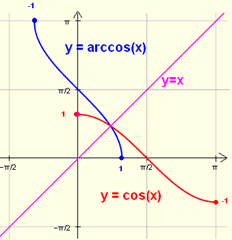
\includegraphics[width=0.35\columnwidth]{pic2.png}
		\end{center}
\pagebreak	
%\begin{flushleft}
	\subsection{Arccos Table}
%\end{flushleft}
The below table contains some of the commonly calculated values of	x for various angles($\theta$) in Radian(Rad) \& Degrees($^{\circ}$).
	\begin{center}
		\begin{tabular}{|c|c|c|}
			\hline
			x&arccos(x)&arccos(x)\\
			 &(Rad)&($^{\circ}$)\\
			 \hline
			 -1&$\pi$&180$^{\circ}$\\
			 \hline
			 -$\sqrt{3}$/2&5$\pi$/6&150$^{\circ}$\\
			 \hline
			 -$\sqrt{2}$/2&3$\pi$/4&135$^{\circ}$\\
			 \hline
			 -1/2&2$\pi$/3&120$^{\circ}$\\
			 \hline
			 0&$\pi$/2&90$^{\circ}$\\
			 \hline
			1/2&$\pi$/3&60$^{\circ}$\\
			 \hline
			 $\sqrt{2}$/2&$\pi$/4&45$^{\circ}$\\
			 \hline
			 $\sqrt{3}$/2&$\pi$/6&30$^{\circ}$\\
			 \hline
			 1&0&0$^{\circ}$\\
			 \hline
		\end{tabular}
	\end{center}
	
	\pagebreak
	\begin{center}
		\section{Problem-2} 		
	\end{center}
		\subsection{Problem Statement}

		To develop a system in Java to calculate the result for the trigonometric function arccos(x).
		
	\begin{flushleft}
		\subsection{Requirements}
		\small (Requirements are denoted by unique identifiers preceeding with 'R'.)
	\end{flushleft}
	Below are few constraints that need to be followed:
	\begin{itemize}
		\item[R1.] \textbf{Interface requirement:} The system(function) shall interact with the user for input needed for start of computation.
		\item[R2.] \textbf{Quality requirement:} The system shall be flexible, reliable, reusable and maintainable due to the complex nature of calculations involved.
		\item[R3.] \textbf{Functional requirement:} The system shall display appropriate error messages/have appropriate error handling mechanism to ensure understanability to the user in case of incorrect input given.
	\end{itemize}
		
	\begin{flushleft}
		\subsection{Assumptions}
		\small (Constraints are denoted by unique identifiers preceeding with 'C'.)
	\end{flushleft}
		Below are few constraints that need to be followed:
		\begin{itemize} 
			\item[C1.] The user shall input the value of x in the range of -1$\leq$x$\leq$1.
			\item[C2.] The value of $\pi$ upto 10 decimal places shall be considered for computation and related calculations.
		\end{itemize}
\pagebreak
	\begin{center}
		\section{Problem-3} 		
	\end{center}
		\subsection{Algorithm 1-Pseudocode}
		This program allows users to calculate the inverse of cos(arccos) for a variable x and fetch the respective measure in degrees using the \textbf{Taylor series expansion formula}.\\\\
		\textbf{function power(argument1,argument2)\{}\\
			Calculates the result for $(argument1)^{argument2}$\\
			if argument1 is equal to 0\par
			\vspace{-0.3cm}return undefined error\\
			else if argument2 is equal to 0\par
			\vspace{-0.3cm}return 1\\
			else\par
			\vspace{-0.3cm}return the value of first argument raised to the power of second argument\\
			end\\
		\textbf{\}}\\\\
		\textbf{function factorial(argument1)\{}\\
			Calculates the factorial(n!) of the passed argument\\
			Check the validity of the argument\\
			if argument1 less than 0\par
			\vspace{-0.3cm}return undefined error\\
			else if argument1 is equal to 0\par
			\vspace{-0.3cm}return 1\\
			else\par
			\vspace{-0.3cm}return the factorial of the passed argument\\
			end\\
		\textbf{\}}\\\\
		\textbf{function acos(argument1)\{}\\
			Calculates the inverse of cosine(arccos) for a variable in the range of [-1,1] using the Taylor series expansion formula:\\\\
			$arccos(x)=\frac{\pi}{2}-arcsin(x)$\\
			$arccos(x)=\frac{\pi}{2}-\sum_{n=0}^{\infty}\frac{2n!}{2^{2n}(n!)^2}\frac{x^{2n+1}}{2n+1}$ which converges for -1$\leq$x$\leq$1\\\\
			if argument1 is less than -1 or greater that 1\par
			\vspace{-0.3cm}return invalid input error\\
			else\par
			\vspace{-0.3cm}Call the factorial and power function to perform the appropriate calculations\\
			return the inverse of cosine(arccos(x))\\
			end\\
			\textbf{\}}\\\\\\
			\textbf{\{}\\
				In the \textbf{main function}\\
				Print prompt “Input the value of variable for finding arccos”\\
				Take the input from user\\
				Send the input to the acos function and display the result for the user\\
			\textbf{\}}\\
			
		The above algorithm is the most accurate of the 2 algorithms in this section. This algorithm is distributed into various functions thereby using the core object oriented principles of Java such as polymorphism and encapsulation. The more the number of iterations in the formula, the lesser would be the error coefficient. It also makes use of recursion to find the factorial of the numbers needed in the formula.
	\subsection{Algorithm 2-Pseudocode}	
	This program allows users to calculate the inverse of cos(arccos) for a variable x and fetch the respective measure in degrees using the Chebyshev-Pade quotient approximation.\\\\
	\textbf{function acos(argument)\{}\\
		if argument is less than -1 or greater than 1\par
		\vspace{-0.3cm}return invalid input error\\
		else\par
		\vspace{-0.3cm}calculate result using the following Chebyshev-Pade quotient approximation:\\
		result = $\frac{\pi}{2}-(0.5689111419 - 0.2644381021*argument-0.4212611542*(2*argument - 1)*(2*argument - 1)+0.1475622352*(2*argument - 1)*(2*argument - 1)*(2*argument - 1))/(2.006022274 - 2.343685222*argument + 0.3316406750*(2*argument - 1)*(2*argument - 1)+0.02607135626*(2*x - 1)*(2*x - 1)*(2*x - 1))$\\
		\vspace{0cm}
		end\\
	\textbf{\}}\\\\
	\textbf{\{}\\
	In the \textbf{main function}\\
	Print prompt “Input the value of variable for finding arccos”\\
	Take the input from user\\
	Send the input to the acos function\\
	\textbf{\}}\\\\
	The above algorithm is a simpler approximation of arccos(x) with lesser memory utilization and load on JVM. Being directly associated with approximated quotients, the calculations are lighter and easy to compute.
	
	\subsection{Advantages vs Disadvantages}
	\begin{center}
		\begin{tabular}{p{8cm}|p{8cm}}
			\textbf{\underline{Pseudocode-1}}&\textbf{\underline{Pseudocode-2}}\\
			\textbf{Advantages}: 1. Accuracy is more than pseudocode-2 with an error coefficient of $\approx$ 0.6-0.7 off the original value. &\textbf{Advantages}: 1. The simplest of implementation since the code involves mostly constants which do not need to be computed separately.\\
			2. Better readability and understandability of code due to the disctribution of various critical functions rather than have a congestion of information(or code).&2. Less intensive on the JVM due to the need of only a single function for the end output computation.\\
			\textbf{Disadvantages}: 1. Lengthier implementation of code and possibility of error in logic due to the need of various functions for end output.&\textbf{Disadvantages}: 1. The error coefficient is the major concern due to difference of $\approx$ 7-8 degrees off the original value.
		\end{tabular}
	\end{center}

\section{References}
\begin{enumerate}
	\item[i.] http://mathworld.wolfram.com/Cosine.html
	\item[ii.] https://www.analyzemath.com/Graphing/graphing\_arccosine.html
	\item[iii.] https://en.wikipedia.org/wiki/Inverse\_trigonometric\_functions
	\item[iv.] https://www.rapidtables.com/math/trigonometry/arccos.html\#definition
	\item[v.] https://ieeexplore.ieee.org/document/8559686
	\item[vi.] https://www.mathportal.org/formulas/pdf/taylor-series-formulas.pdf
	\item[vii.] https://cs.uwaterloo.ca/~kogeddes/papers/Numapprox/Numapprox.html
\end{enumerate}
		
	
\end{document}